\section{Simulation results and comparison}\label{sec:ch6_results}

We illustrate our work using the motivating case study of a vision-based lateral control system explained in Section~\ref{sec:lkas_case_Study} and described as follows.
\begin{equation}
\label{eq:ch6_lkasmodel}
\vspace{-1em}
     \dot x(t) = \Acont (v_x) x(t) + \Bcont u(t - \tau),\ 
     y(t) = \Ccont x(t),
\end{equation}

\subsection{\Gls{mpc} implementation}
Based on a discretized version\footnote{The symbolic math toolbox of MATLAB R2015b was used for obtaining the required discrete-time \gls{lpv} model from~\eqref{eq:ch6_lkasmodel}} of~\eqref{eq:ch6_lkasmodel} using methods discussed in Section~\ref{sec:ch6_discmodel}, the optimization problem~\eqref{eq:ch6_mpcopt} can be formulated for \gls{mpc} with longitudinal velocity $v_x$ and delay parameter $n_d$ as the scheduling variables. Constraints are imposed on the control input $\delta_f$. In~\eqref{eq:ch6_predmodeleqs}, $v_x$ may be assumed either to be a constant in prediction or a variable, as described in Section~\ref{sec:ch6_probform}. Since for the considered lateral control system, problem~\eqref{eq:ch6_mpcopt} has a quadratic cost function subject to linear constraints, it can be solved using any \gls{qp} algorithm. We use the methods described in~\cite{sparseNMPC} for an efficient implementation. Specifically, the \gls{qp} problem~\eqref{eq:ch6_mpcopt} is transformed to the following box-constrained least-squares problem by eliminating equality constraints through quadratic penalties with large weight $\rho$, i.e.,
\begin{align}
    &\resizebox{0.8\textwidth}{!}{$\min\limits_{u(\cdot), y(\cdot)} J(k) + \rho \sum\limits_{l=1}^{N_{\text{p}}} \left\Vert y(k+l)-M(p, n_d(k))  \cdot\phi(k+l-1)\right\Vert^2 $}\label{eq:ch6_bvls} \\
  &\text{s.t.\ \eqref{eq:ch6_ybounds}-\eqref{eq:ch6_ubounds}}, %\notag
\end{align}
and by substituting~\eqref{eq:ch6_ctrlhor}-\eqref{eq:ch6_initphi} in the cost function. Following~\cite{sparseNMPC}, we implement the optimization algorithm such that it is not only able to automatically adapt to changes in parameters $p$ including $n_d$ but also \gls{mpc} parameters such as the horizons $N_{\text{u}}$, $N_{\text{p}}$, and the tuning weights through which the controller can be re-tuned at run time. Besides this, as problem~\eqref{eq:ch6_bvls} is always solvable, this method has a practical benefit as it is also able to deal with situations under which the constrained \gls{qp}~\eqref{eq:ch6_mpcopt} might become infeasible to solve due to model mismatch and unmeasured disturbances.

\begin{table*}[t]
\centering
\caption{Comparison between the proposed pipelined \gls{spade} \gls{mpc} approach with the state-of-the-art multiprocessor \gls{ibc} system implementations}
\label{tab:ch6_my-table}
\resizebox{\textwidth}{!}{
\begin{threeparttable}	
\begin{tabular}{|p{2.9cm}|p{3cm}|p{3cm}|p{3cm}|p{3cm}|}
\hline
\multicolumn{1}{|c|}{\multirow{2}{*}{Criteria}} &
  \multicolumn{1}{c|}{\multirow{2}{*}{\gls{spade} pipelined \gls{mpc}}} &
  \multicolumn{2}{c|}{Pipelined} &
  \multirow{2}{*}{Chapter \ref{chap:parallelisation}} \\ \cline{3-4}
\multicolumn{1}{|c|}{} &
  \multicolumn{1}{c|}{} &
  \multicolumn{1}{c|}{constant delay~\cite{medina2019designing},~\cite{krautgartner1998performance}} &
  \multicolumn{1}{c|}{variable delay~\cite{medina2019implementation}} &
   \\ \hline
Inter-frame dependencies    & explicitly considered   & not considered           & not considered         & independent          \\ \hline
System nonlinearities                & explicitly considered    & not considered     & not considered   & not considered \\ \hline
Constraints on variables               & can be strictly imposed    & cannot be imposed     & cannot be imposed   & cannot be imposed \\ \hline
Control computation time                 & high (worst-case up to 15x greater than Chapter \ref{chap:parallelisation})    & low  & medium (a delay predictor needed)   & low (feedback gain matrix multiplication) \\ \hline
Algorithm                 & white/gray/black box    & white/gray/black box     & white/gray/black box   & white/gray box \\ \hline
Parallelisation potential & independent             & independent              & independent            & should be high       \\ \hline
Workload variations       & explicitly considered in design             & not considered           & indirectly considered as variable delay   & explicitly considered in design \\ \hline
Platform                  & suitable for homogeneous  & suitable for homogeneous & can be adapted for all & directly applicable for all   \\ \hline
Restrictions on $h$\tnote{1}      & strictly periodic; $h < \tau_{wc}$  &  strictly periodic; $h < \tau$    &  strictly periodic; $h < \tau_{wc}$  & switched system possible
\\ \hline
Restrictions on $\tau$  & strictly\tnote{2}\ $\ \tau_{wc}>h$    & strictly $\tau > h$; in~\cite{medina2019designing}, $\tau$ is strictly a multiple of $h$ & strictly\tnote{2}\ $\ \tau_{wc}>h$  & $\tau_{wc} \le h$   \\ \hline
\end{tabular}%
\begin{tablenotes}
			\footnotesize
			\item{$\tau_{wc}$: worst-case delay;\ $^1$ If camera frame arrival period $\fh$ is considered, always $h$ is a multiple of $\fh$; $^2$ if $\tau\le h$ design reverts to sequential; } 
		\end{tablenotes}
		\end{threeparttable}
}
\vspace{-2em}
\end{table*}

\subsection{Controller performance evaluation}
This section includes simulation results for our case study. We consider two scenarios: 1) the adaptive \gls{mpc} algorithm is run with 
a constant worst-case delay, i.e. neglecting workload variations, and 2) with delay as a variable to explicitly consider workload variations, without changing any tuning parameters.
The purpose of this simulation is to highlight the benefits of the control design that also adapts well with workload variations. The influence of delay is apparent with model mismatch and unmeasured disturbances. Since the true system considered is the continuous-time model~\eqref{eq:ch6_lkasmodel} and discretization errors are negligible, in order to emulate the influence of realistic model mismatch and unmeasured disturbances, we provide the output reference for vehicle lateral control along with the output measurement, i.e., with a varying delay. Note that this is done only for this particular simulation scenario and is not the case in practice where the reference is already known.

We assume the camera frame rate of 60 fps, i.e., $\fh=1/60$ s. Simulation length is 5000 time steps i.e.\ $T=83.33$ s. Unit weights are imposed on all \gls{io} variables for \gls{mpc}, while $N_{\text{p}}=N_{\text{u}} = 10$ time steps. The steady-state input reference $u_r(t)=0$ whereas the output reference profile is set to a sinusoidal signal such that at time step $k$, $y_r(k)=2.5\cdot \sin{(5kh\pi/T)} $ m. The longitudinal velocity is a ramp signal such that $v_x(0)=45$ and $v_x(T) = 80$ km/h, which we assume to be known in prediction for the controller. 

The mean runtime for the control algorithm was 2.2~ms while solving the optimization problems with 20 decision variables in MATLAB (on a computer equipped with a 2.6GHz processor). Referring to the reported runtimes in~\cite{sparseNMPC} for control problems of comparable size, we expect a similar efficient embedded implementation of the algorithms with a C backend to significantly reduce these runtimes (roughly by 20x, to about 0.1~ms) on a processor with comparable specifications. Assuming that the target platform is around 60 times slower, the \gls{wcet} of tasks \taskS, \taskC\ and \taskA\ are $\actorET_{\taskS}$=~60~ms (based on Chapter \ref{chap:parallelisation}), $\actorET_{\taskC}$=~6~ms~\cite{sparseNMPC} and $\actorET_{\taskA}$=~0.5~ms, respectively. This results in worst-case delay $\tau=66.5$~ms and $n_f=4$.
\begin{figure}[t]
    \centering
    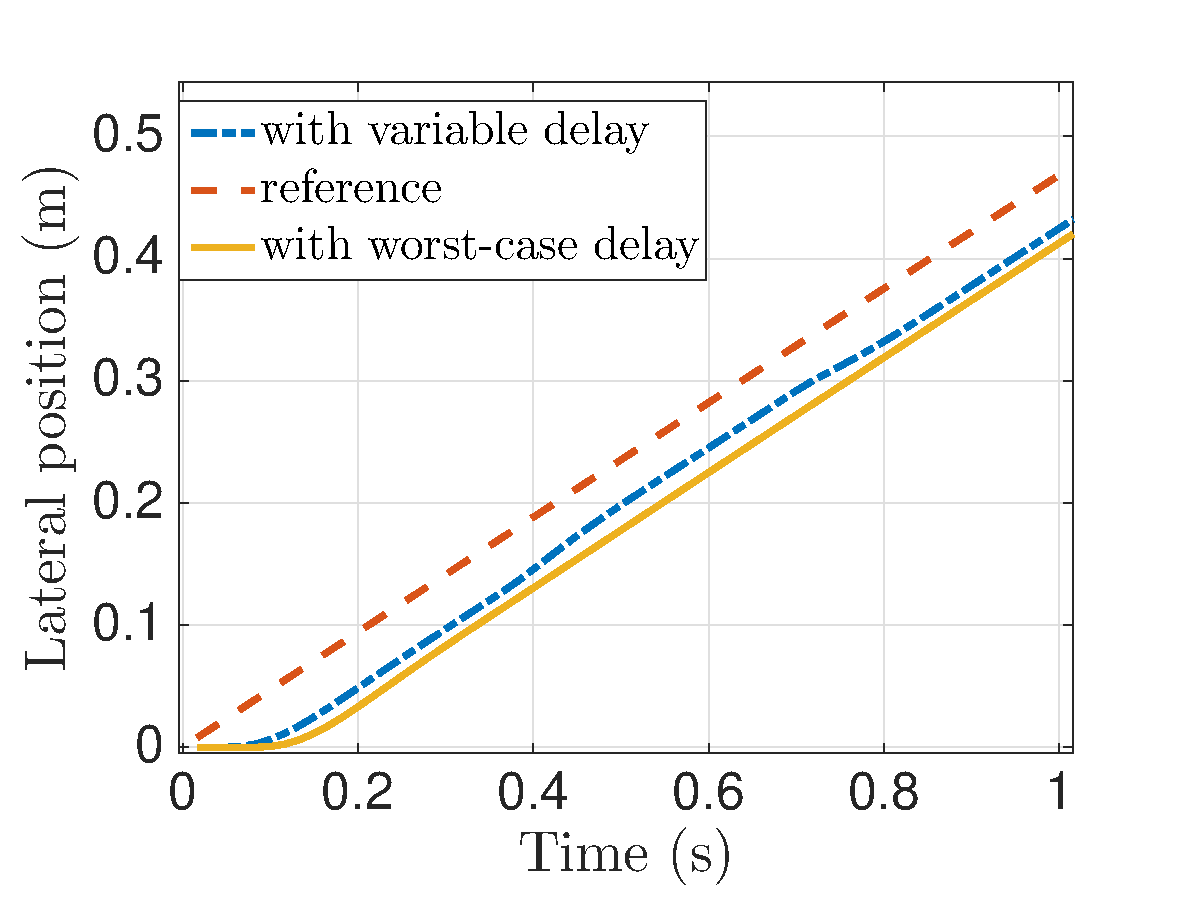
\includegraphics[height=0.5\linewidth]{images/simresults3.eps}
    \caption{Lateral position of the vehicle w.r.t.\ the road centre.}
    \label{fig:ch6_comparison}
    \vspace{-2em}
\end{figure}

We assume that the inter-frame dependence time $\fd$ is given and $\fd=15$ ms. 
So $n_s=1$ and the maximum number of cores needed $\maxCores=4$.
We assume that $\numCoresAvailable=4$ and thus $h=1/60$ s.
To simulate the workload variations for the variable delay scenario, we consider the delay to be a random signal where the delay may take any value $n_d h$ which is held constant for every 20 frames such that $n_d\in\{1,2,3,4\}$ with the corresponding probability distribution of occurrence as \{0.2435,0.3534,0.3073,0.0958\}. Such a probability distribution for characterising workload variations can be statistically analysed from observed data~\cite{fontantelli2013optimal}.

Based on the aforementioned simulation implemented in MATLAB on a computer equipped with a 2.6GHz processor, the results obtained show that a \gls{rmse} of 2.98~cm from the output reference is achieved using \gls{mpc} considering a variable delay. 
For \gls{mpc} based on constant (worst-case) delay the \gls{rmse} increases by 26.85\% to 3.78~cm, as is clearly seen in Fig.~\ref{fig:ch6_comparison}. The improvement by handling workload variations is expected to be higher when the worst-case delay is considerably larger than its mean. 

In the simulation, we considered the following aspects which are crucial for real-life practical implementation. 1) inter-frame dependencies: $\fd=15$ ms; 2) system nonlinearities: $v_x$ is a ramp signal; 3) constraints: $\delta_f$ constrained to maximum magnitude of 0.5 radians; and 4) workload variations as a variable delay based on probability distribution. 

\subsection{Comparison with the state-of-the-art}
We compare the proposed \gls{mpc} formulation for pipelined \gls{ibc} implementation with state-of-the-art multiprocessor \gls{ibc} design techniques in Table~\ref{tab:ch6_my-table}. 
For brevity, we only compare with multiprocessor \gls{ibc} system implementations and not with traditional sequential control design techniques based on the worst-case sensing delay, as it has already been shown in~\cite{fontantelli2013optimal} that considering workload variations is beneficial for optimizing control performance.
The multiprocessor implementations can be classified into pipelined~\cite{medina2019designing},~\cite{krautgartner1998performance} with constant delay, pipelined with variable delay~\cite{medina2019implementation} and sequential implementation with parallelisable sensing (explained in Chapter~\ref{chap:parallelisation}).
The camera frame rate, however, is not explicitly considered in~\cite{krautgartner1998performance}.

The proposed approach is advantageous to others with respect to: 1) considering inter-frame dependencies; 2) modelling and considering system nonlinearities; and 3) strictly imposing constraints on the system variables. 
These aspects are crucial for practical implementation and explicitly considering them helps in making a step forward towards real-life adaptation.
The proposed approach, however, requires higher worst-case control computation time $\actorET_\taskC$ (up to 15x greater than in Chapter \ref{chap:parallelisation}) due to solving the online optimization problem.
Note that $\actorET_\taskC$ is not yet significant compared to the sensing workload, i.e., ${\actorET_\taskS \gg \actorET_\taskC+\actorET_\taskA}$.
Future work includes identifying a case where $\actorET_\taskC$ can be significant compared to the sensing workload and adapting our method for it.